\documentclass[11pt, oneside]{article}   	% use "amsart" instead of "article" for AMSLaTeX format
\usepackage{geometry}                		% See geometry.pdf to learn the layout options. There are lots.
\geometry{letterpaper}                   		% ... or a4paper or a5paper or ... 
%\geometry{landscape}                		% Activate for for rotated page geometry
%\usepackage[parfill]{parskip}    		% Activate to begin paragraphs with an empty line rather than an indent
\usepackage{graphicx}				% Use pdf, png, jpg, or eps§ with pdflatex; use eps in DVI mode
								% TeX will automatically convert eps --> pdf in pdflatex		
\usepackage{amssymb}
\usepackage{latexsym}
\usepackage{qtree}
\usepackage{graphicx,pdflscape}
\usepackage{tikz}
\usepackage{tikz-qtree}
\usepackage{comment}
\usepackage{multirow}
\usepackage{subfigure}
\usepackage{algorithm}
\usepackage{algpseudocode}

\title{CS689 Sampling-Based Motion Planning Report}
\author{Zhonghua Xi}
%\date{}							% Activate to display a given date or no date

\begin{document}
\maketitle

\section{MyApproach}
My approach to expend the tree is a variant of RRT with two main differences.
\begin{enumerate}
  \item Maximum Expansion Distance 
  \item Obstacle Based
\end{enumerate}
Since it was inspired from the bug algorithm, let us call it B-RRT.

\subsection{Maximum Expansion Distance}
Instead of expend as far as possible, 
B-RRT will only expend at most certain amount of distance called maximum extending distance (MED), which was set to 20\% of the diagonal of the bounding box for experiment and could be a user given parameter.
This approach try to avoid extending in open space since we don't want to explore the space that are entirely free.

\subsection{Obstacle Based}
During expansion, once the robot hit an obstacle, 
instead of stop expansion and generate a new random configuration, 
B-RRT will continue expending the tree from the last valid configuration expended in both directions that are perpendicular to the original expansion direction with MED$'$ which was set to 10\% of MED.
This strategy gives B-RRT the ability to explore the boundary area very quickly without sampling. 

\subsection{Pseudocode}
Pseudocode of ExtendTree and ExtendBRRT are given in Alg.~\ref{alg:extendTree} and Alg.~\ref{alg:extendBRRT}.
In which MES and MES$'$ are maximum extending steps and are computed according to MED and MED$'$.

\begin{algorithm}                      	
\caption{ExtendTree($q$, $q_{rand}$, $steps$)}
\label{alg:extendTree}                     	
\begin{algorithmic}
\State $d \gets (q_{rand} - q) / DistOneStep$
\State $MaxStep \gets min(|q_{rand} - q| / DistOneStep, steps)$
\State $q_{last} \gets NULL$
\For {$i \gets 1$ to MaxStep}
	\State $q_{new} \gets q + i*d$
	\If {$IsValid(q_{new})$}
    	\State $AddVertex(q_{new})$
		\State $q_{last} \gets q_{new}$ 
	\Else
    	\If {$i \ne MaxStep$}
        	\State	\Return $q_{last}$
    	\EndIf
	\EndIf
\EndFor
\State \Return $NULL$
\end{algorithmic}
\end{algorithm}

\begin{algorithm}                      	
\caption{ExtendBRRT}
\label{alg:extendBRRT}                     	
\begin{algorithmic}
\State {$q_{rand} \gets GetRandomConfig()$}
\State {$v_{closest} \gets GetClosestVertex(q_{rand})$}
\State {$v_{last} \gets ExtendTree(v_{closest}.pos, q_{rand}, MES)$}
\If {$v_{last} \ne NULL$}
	\State $q \gets GetPerpendicular(q_{rand} - v_{closest}.pos)$
	\State $ExtendTree(v_{last}.pos, q*scale, MES')$
	\State $ExtendTree(v_{last}.pos, -q*scale, MES')$
\EndIf
\end{algorithmic}
\end{algorithm}

\subsection{Advantages}
Identical or faster than RRT in normal cases, and much faster in narrow passage cases (1.91x in Scene 6). 
Trees generated by RRT and B-RRT are shown in Figure.~\ref{fig:trees}, 
from which we can see that, B-RRT generates fewer nodes in the open space (left-up and left-bottom corners) than RRT does.

\subsection{Disadvantage}
The B-RRT tree doesn't look pretty, RRT's properties may not guaranteed locally.

\begin{figure}[h!]
  
  \centering
    \subfigure[RRT]{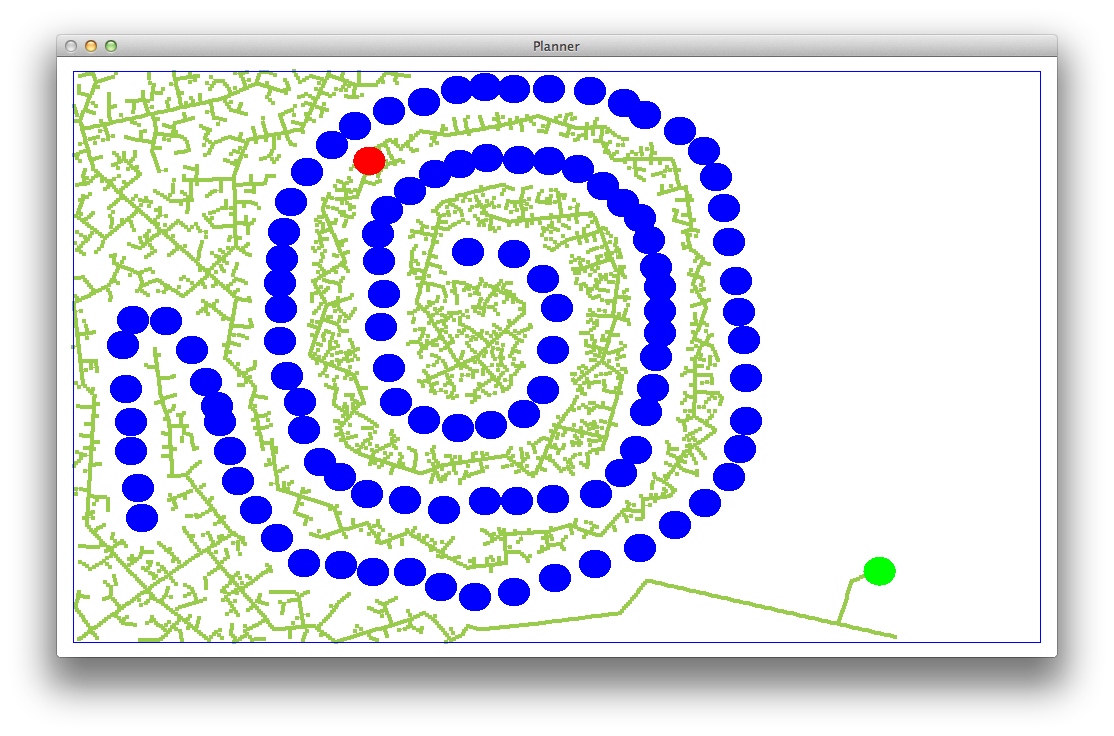
\includegraphics[width=0.48\textwidth, clip=true, trim=20mm 27mm 20mm 20mm]{rrt.png}}
    \subfigure[B-RRT]{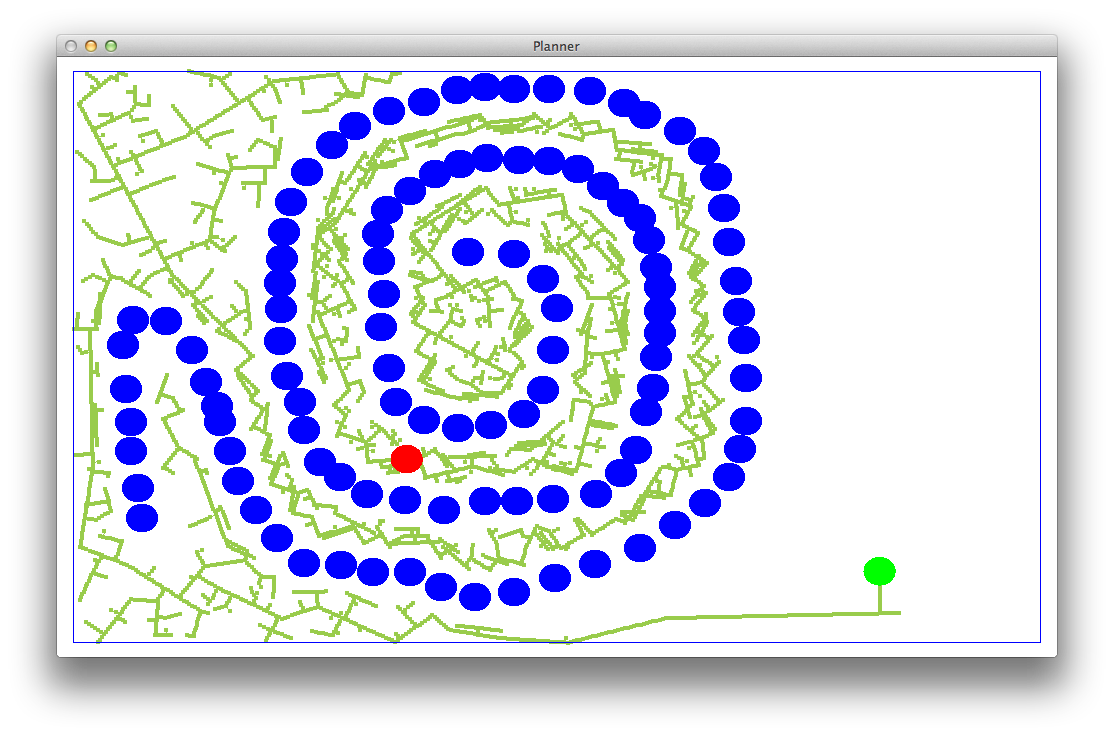
\includegraphics[width=0.48\textwidth, clip=true, trim=20mm 27mm 20mm 20mm]{brrt.png}}
  \caption{Trees generated by RRT and B-RRT on Scene 6.}
  \label{fig:trees}
\end{figure}



\section{Comparison}
Comparison on running time and size of the tree for each algorithm is shown in Table~\ref{tab:running-time}. 
Time limit for solving the problem was set to 30 seconds. 
Every number reported in Table~\ref{tab:running-time} is the average result of 30 runs.
All data are collected on a 2012 MacBook Pro Laptop, with a 2.9GHz Intel i7 CPU and 16GB RAM.

\begin{table}
\begin{center}
    \begin{tabular}{ | c | c | c | c | c |}
    \hline
    Scene 					& Method 	& Success 	& Time (s)						& Nodes 						\\ \hline
    \multirow{4}{*}{1}		& Random 	& 1.00 		& 0.00744 $\pm$	0.00705			& 4361		$\pm$	4186		\\ 
    						& EST		& 1.00		& 0.04601 $\pm$ 0.02426 		& 2388 		$\pm$	782 		\\ 
							& RRT 		& 1.00 		& 0.00039 $\pm$	0.00027 		& 178 		$\pm$	67	 		\\ 
 							& B-RRT		& 1.00		& 0.00031 $\pm$	0.00021  		& 157 		$\pm$	56	 		\\ \hline
    \multirow{4}{*}{2}		& Random 	& 1.00 		& 0.02246 $\pm$	0.02495 		& 13051 	$\pm$	13279	 	\\ 
    						& EST		& 1.00		& 0.07011 $\pm$	0.02851  		& 3508 		$\pm$	763		  	\\ 
							& RRT 		& 1.00 		& 0.00071 $\pm$	0.00064  		& 196 		$\pm$	63	  		\\ 
 							& B-RRT		& 1.00		& 0.00053 $\pm$	0.00031  		& 185 		$\pm$	56	  		\\ \hline
	\multirow{4}{*}{3}		& Random 	& 1.00 		& 2.48902 $\pm$	1.77917  		& 11593989	$\pm$ 	1184269 	\\ 
    						& EST		& 0.97		& 3.13094 $\pm$	6.15135   		& 11454 	$\pm$	8828	   	\\ 
							& RRT 		& 1.00 		& 0.00271 $\pm$	0.00313   		& 291 		$\pm$	100		   	\\ 
 							& Mine		& 1.00		& 0.00282 $\pm$	0.00409   		& 327 		$\pm$	118	   		\\ \hline
	\multirow{4}{*}{4}		& Random 	& 0.00 		& 30.0000 $\pm$	0.00000   		& 8335309 	$\pm$	1052398	 	\\ 
    						& EST		& 1.00		& 2.18282 $\pm$	0.96452    		& 11454 	$\pm$	2291    	\\ 
							& RRT 		& 1.00 		& 0.08953 $\pm$	0.02001    		& 485 		$\pm$	16	    	\\ 
 							& B-RRT		& 1.00		& 0.05816 $\pm$ 0.01385   		& 487 		$\pm$	23	    	\\ \hline
	\multirow{4}{*}{5}		& Random 	& 0.00 		& 30.0000 $\pm$	0.00002    		& 8603476	$\pm$	1258526  	\\ 
    						& EST		& 0.97		& 12.0262 $\pm$	4.56348     	& 31153 	$\pm$	4070	    \\ 
							& RRT 		& 1.00 		& 0.28915 $\pm$	0.07711     	& 973		$\pm$	15	     	\\ 
 							& B-RRT		& 1.00		& 0.24459 $\pm$	0.05830     	& 978 		$\pm$	21	     	\\ \hline
	\multirow{2}{*}{6$^*$}	& RRT 		& 1.00 		& 0.67158 $\pm$	0.17845     	& 4609		$\pm$	347	     	\\ 
 							& B-RRT		& 1.00		& 0.35069 $\pm$	0.12163     	& 4972 		$\pm$	495	     	\\ \hline						
    \end{tabular}
    \caption{Running Time}	
    \label{tab:running-time}					
    $^*$Scene 6 is the same with Scene 4 but have a 0.2 distOneStep instead of 1.0.
    \end{center}
\end{table}


\end{document}